\chapter{Cloud Capacitor}
\label{chap:capacitor}
% ----------------------------------------------------------
A fim de confirmar as hipóteses de eficácia e eficiência do emprego do Processo
de Avaliação de Capacidade descrito no capítulo anterior, bem como da técnica de
Inferência de Desempenho e das Heurísticas de Seleção que dão suporte a esse Processo, 
criamos uma implementação concreta de sua especificação na forma de uma biblioteca
extensível e de um sistema computacional que demonstra seu funcionamento fazendo
a avaliação de uma aplicação real em um provedor de nuvem de infraestrutura.

Demos o nome de CloudCapacitor à biblioteca, implementada como uma \emph{gem} da
linguagem Ruby~\cite{ruby}. Desenvolvemos o sistema computacional Capacitor Web 
para ser uma interface visual para a utilização do CloudCapacitor, usando 
o \emph{framework} Ruby on Rails~\cite{rails}.  

Descrevemos a seguir os detalhes da implementação de cada um e como ambos se
relacionam para oferecer ao usuário a experiência da avaliação de capacidade
de baixo custo e alta precisão prevista pelo Processo proposto, com uma interface
amigável e de fácil utilização.

\section{Cloud Capacitor}
Cloud Capacitor é uma biblioteca para criação de sistemas de avaliação de 
capacidade em ambientes de nuvem de infraestrutura como serviço. Implementa as
atividades descritas na especificação do Processo de Avaliação de Capacidade do 
Capítulo~\ref{chap:processo}, permitindo que sejam customizadas as atividades
definidas pelo Processo como pontos de extensão, como as Estratégias de Avaliação
e o disparo e controle da execução da Aplicação sob Teste.

implementadas lógicas customizadas de avaliação do desempenho resultante
da execução da Aplicação sob Teste. Essas lógicas são então reconhecidas pelo Cloud 
Capacitor como Estratégias de Avaliação.

\begin{figure}[htb]
  \caption{\label{fig_arq_alto_nivel}Arquitetura de alto nível do Cloud Capacitor}
  \begin{center}
    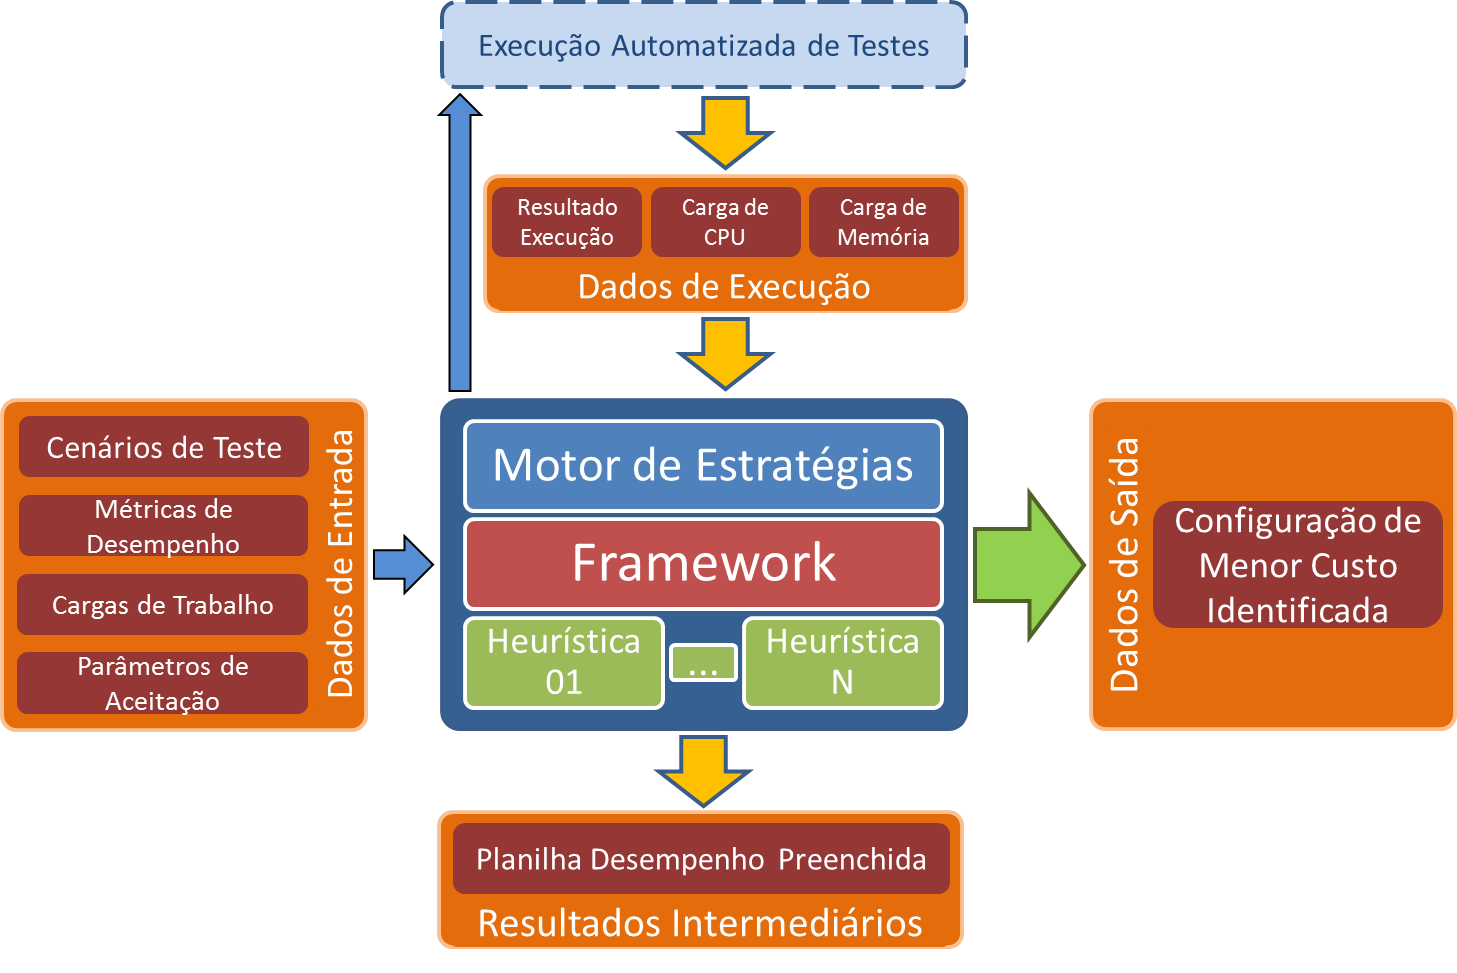
\includegraphics[scale=0.5]{img/arquiteturaAltoNivel}
  \end{center}
\end{figure}

****RASCUNHO
\subsection{Heuristicas}
Para que uma Heurística de Avaliação de Capacidade seja compatível no âmbito deste trabalho, 
deve apresentar um conjunto mínimo de operações esperadas para que a lógica da
avaliação se complete e o resultado final obtido possa ser considerado válido e
comparável com os resultados obtidos por outras Heurísticas.

Além disso, as operações constituem a interface pela qual o controlador das 
sessões de avaliação pode configurar as Heurísticas e informar-lhe os dados 
necessários ao controle da sua execução.
 
Apresentamos esse conjunto mínimo de operações nas subseções a seguir, que 
representam o arcabouço necessário para a construção de uma Heurística de 
Avaliação de Capacidade.
 
% ----------------------------------------------------------
